\documentclass[10pt]{article}
\usepackage[polish]{babel}
\usepackage[utf8]{inputenc}
\usepackage[T1]{fontenc}
\usepackage{amsmath}
\usepackage{amsfonts}
\usepackage{amssymb}
\usepackage[version=4]{mhchem}
\usepackage{stmaryrd}
\usepackage{graphicx}
\usepackage[export]{adjustbox}
\graphicspath{ {./images/} }

\title{GIMNAZJUM }

\author{}
\date{}


\begin{document}
\maketitle
\begin{enumerate}
  \item Udowodnij, że równanie \(x^{2}-7 y^{2}=0\) nie ma rozwiązań w liczbach całkowitych.
  \item Rozstrzygnij, dla jakich liczb naturalnych \(n\) liczba \(n^{4}+n^{2}+1\) jest pierwsza.
  \item Dwie świece jednakowej długości wykonano z różnych rodzajów parafiny. Jedna spala się całkowicie w ciągu 9 godzin, a druga w ciągu 6 godzin. Świece zapalono równocześnie. Za ile godzin świeca spalająca się wolniej będzie dwa razy dłuższa od drugiej świecy?
\end{enumerate}

\section*{LICEUM}
\begin{enumerate}
  \item W półokrąg „wpisano" dwa kwadraty, jak na rysunku obok. Jak powinien być położony punkt A, żeby suma pól tych kwadratów była największa?
  \item Rozwiąż układ równań:\\
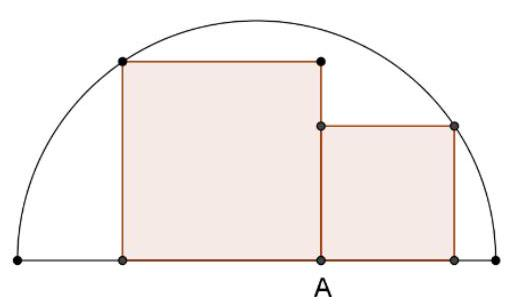
\includegraphics[max width=\textwidth, center]{2024_11_21_1c440a0883d44ee4ee80g-1}
\end{enumerate}

\[
\left\{\begin{array}{l}
x+y+z=14 \\
x+y+t=10 \\
y+z+t=15 \\
x+z+t=12
\end{array}\right.
\]

\begin{enumerate}
  \setcounter{enumi}{2}
  \item Rozwiąż w liczbach całkowitych równanie:
\end{enumerate}

\[
264 x+51 y=20182018
\]


\end{document}